\subsection{User Manual}


\begin{figure}[h]
\captionsetup{justification=centering}
\begin{subfigure}{0.475\textwidth} 
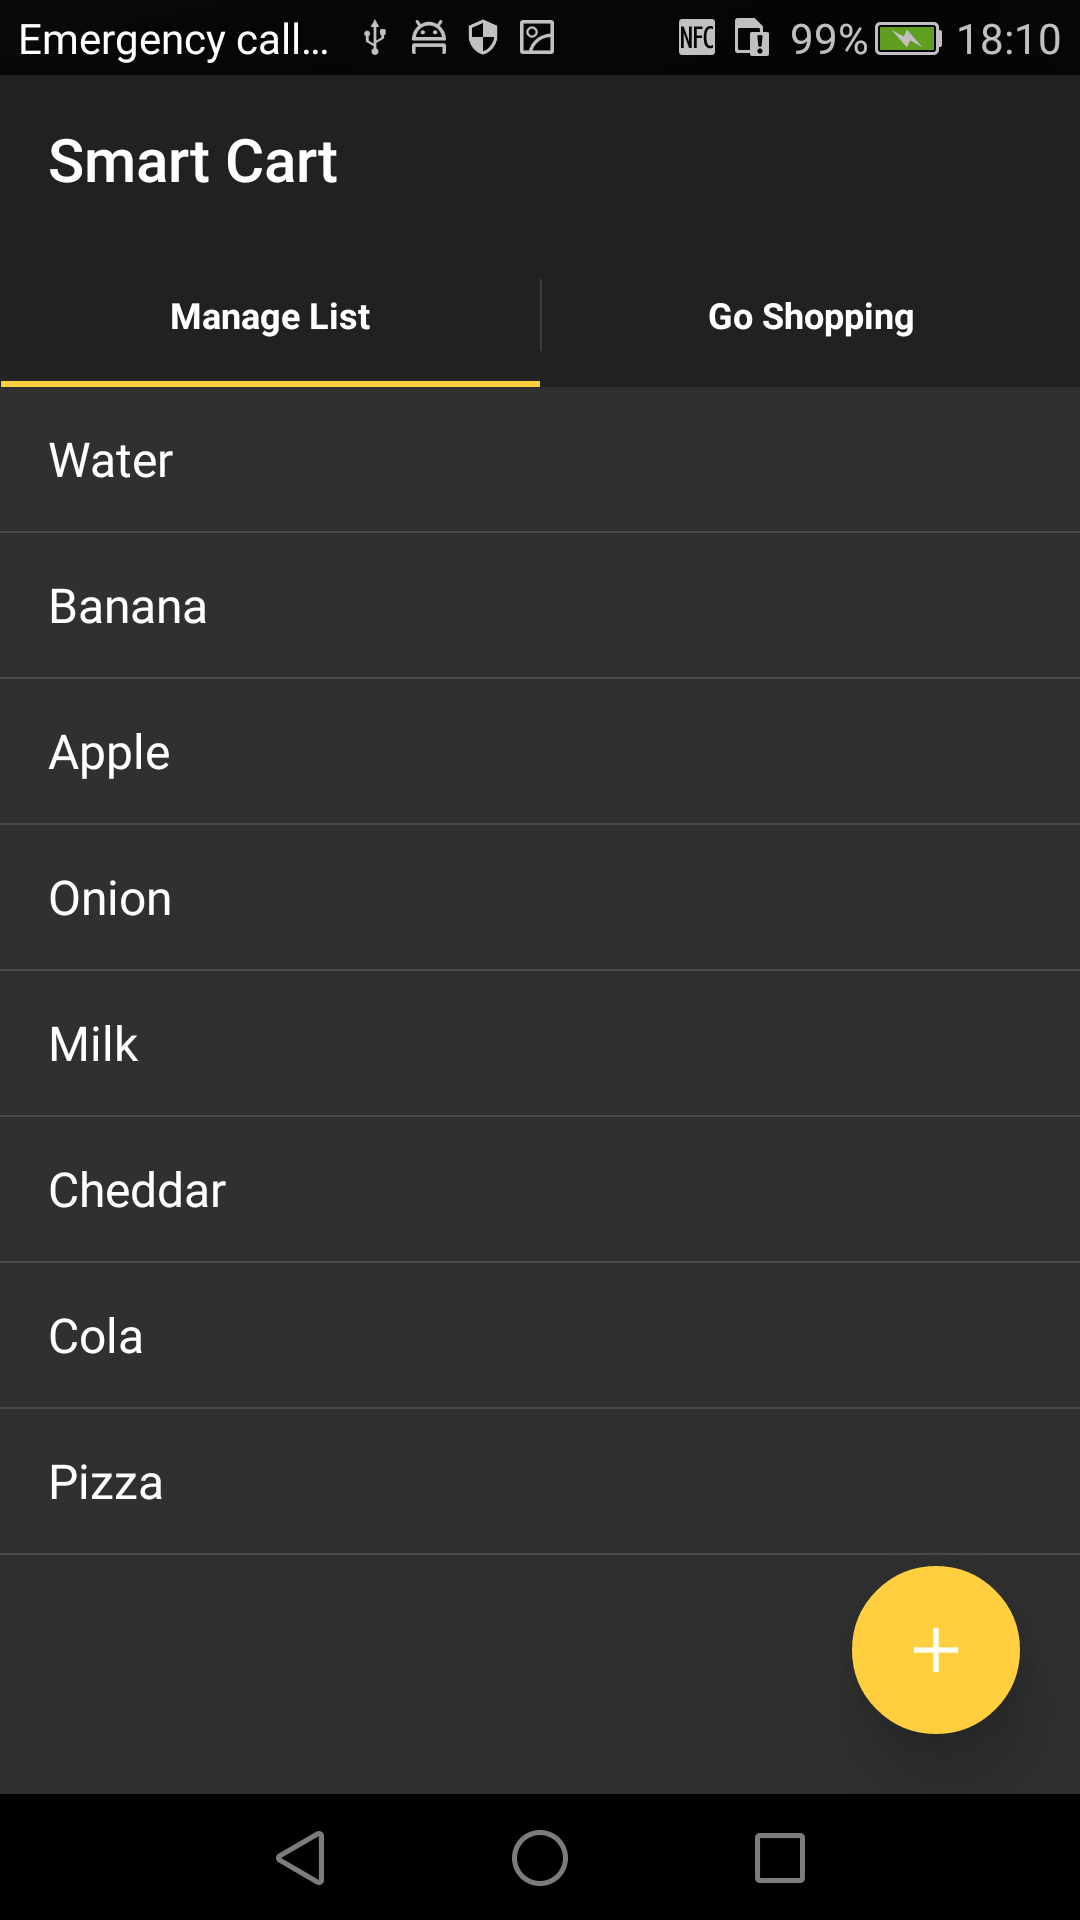
\includegraphics[width=0.8\textwidth, height=
0.35\textheight]{res/usermanual/startApp.png}
\caption{Start}
\label{fig:start}
\end{subfigure} \hspace{0.2\textwidth}
\begin{subfigure}{0.475\textwidth}
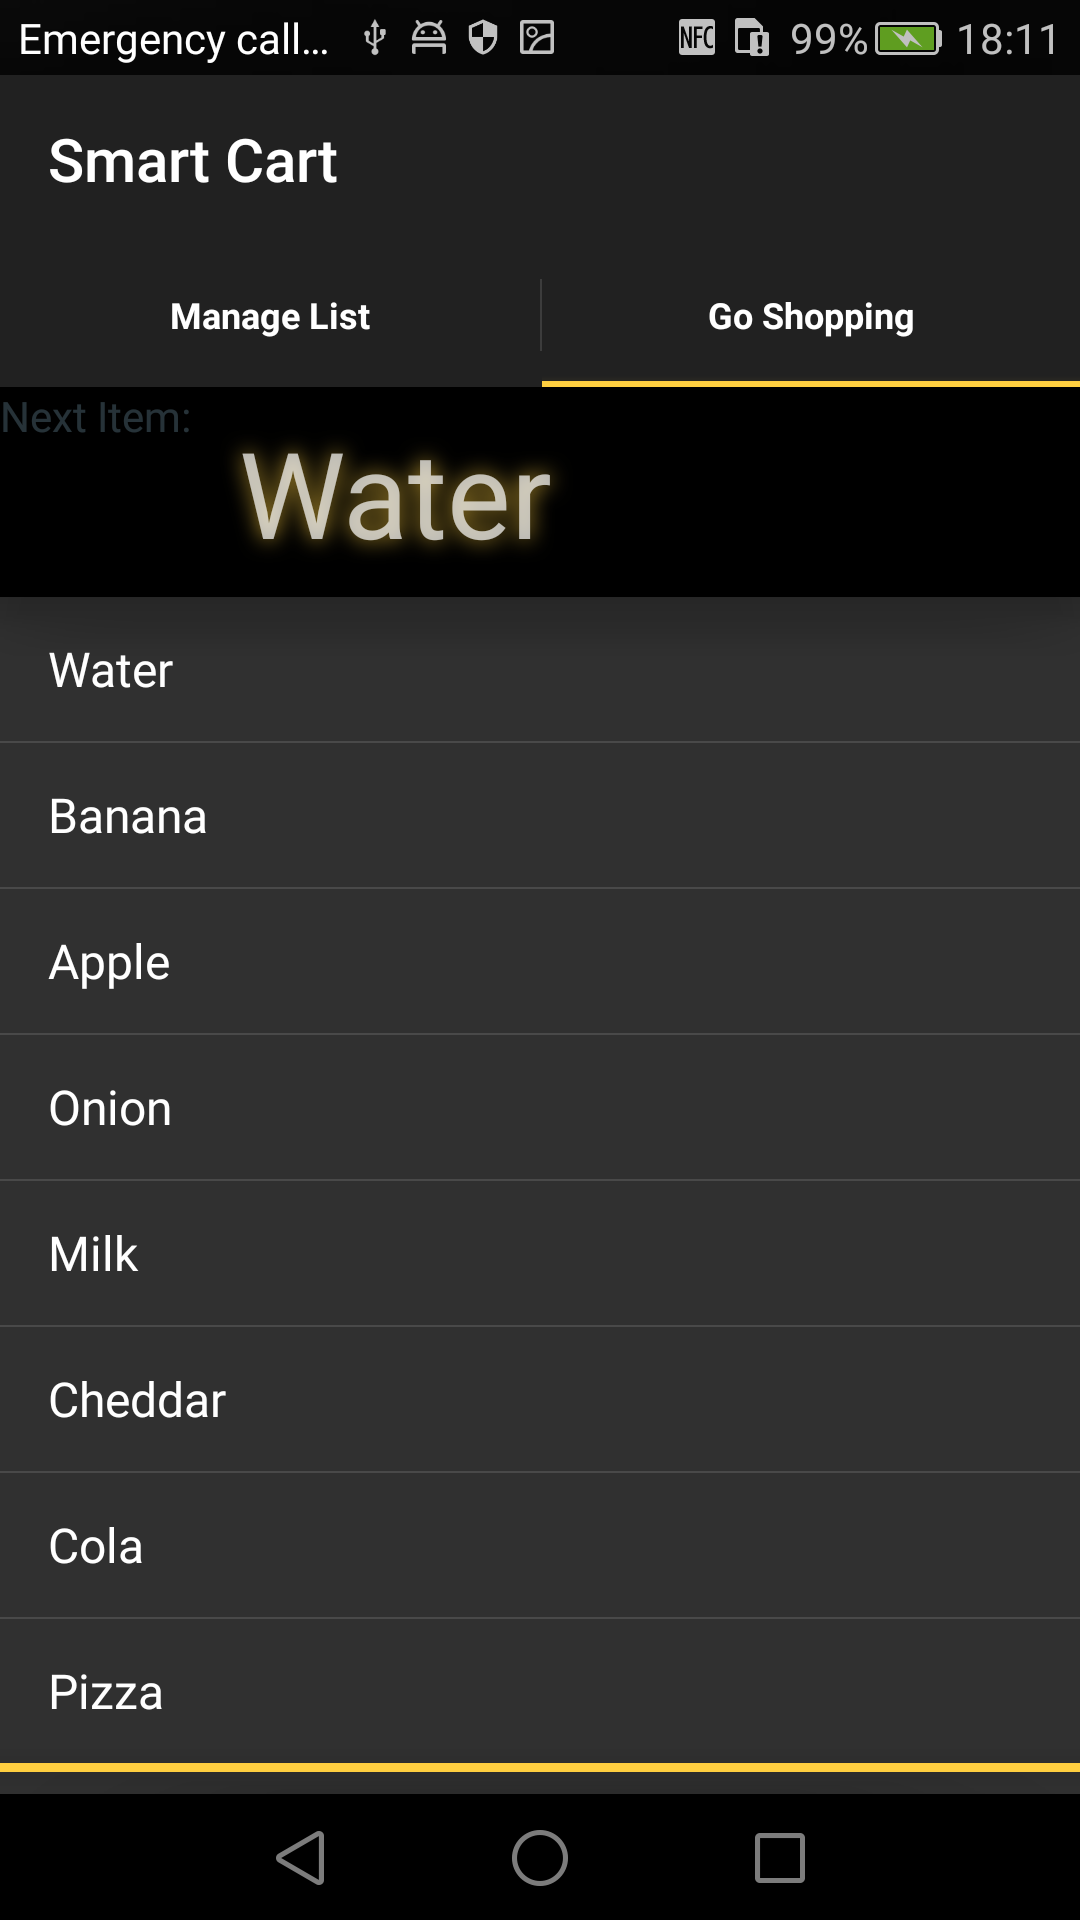
\includegraphics[width=0.8\textwidth, height=
0.35\textheight]{res/usermanual/initialShoppinglist.png}
\caption{Initial Shoppinglist}
\label{fig:initial}
\end{subfigure}
\caption{Initial State after Starting the App}
\label{fig:initialState}
\end{figure}


\begin{figure}[h]
\captionsetup{justification=centering}
\begin{subfigure}{0.475\textwidth} 
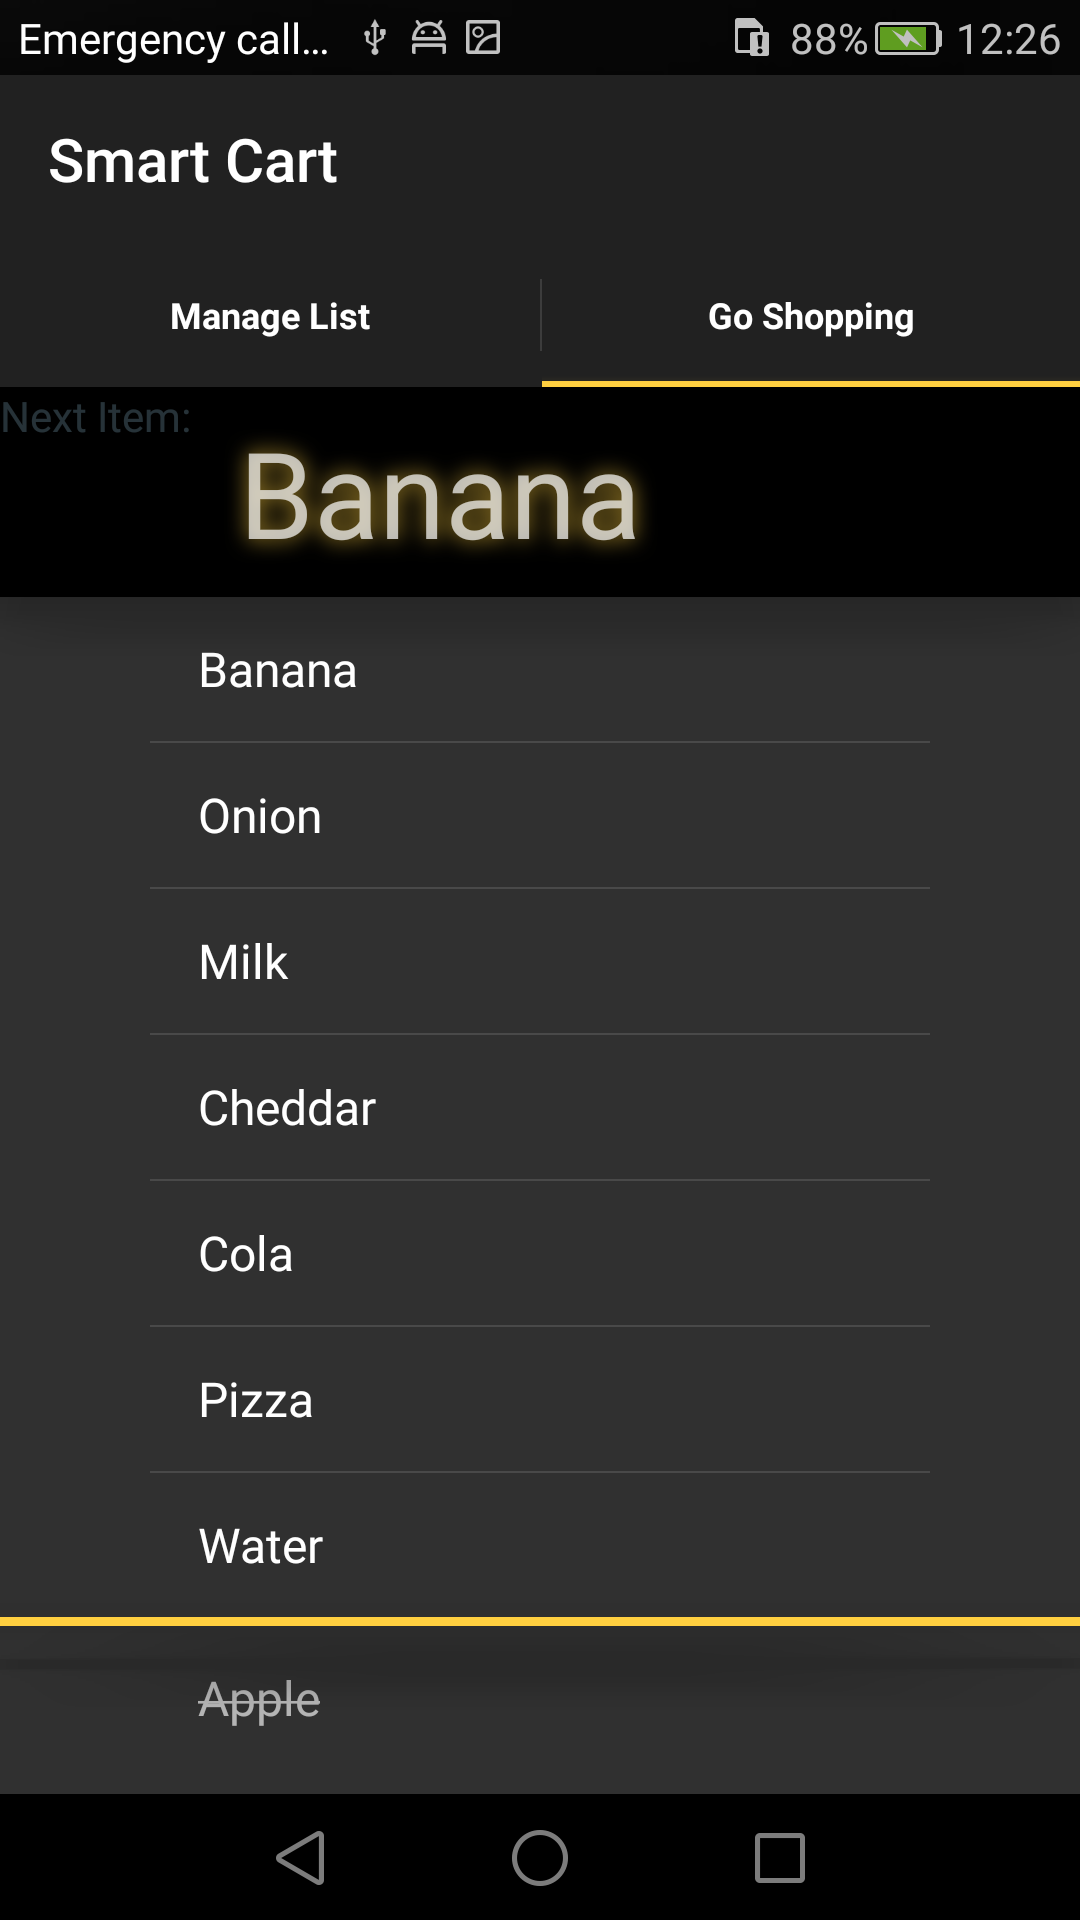
\includegraphics[width=0.8\textwidth, height=
0.35\textheight]{res/usermanual/firstItemChecked.png}
\caption{First Item Checked Off}
\label{fig:firstItemChecked}
\end{subfigure} \hspace{0.2\textwidth}
\begin{subfigure}{0.475\textwidth}
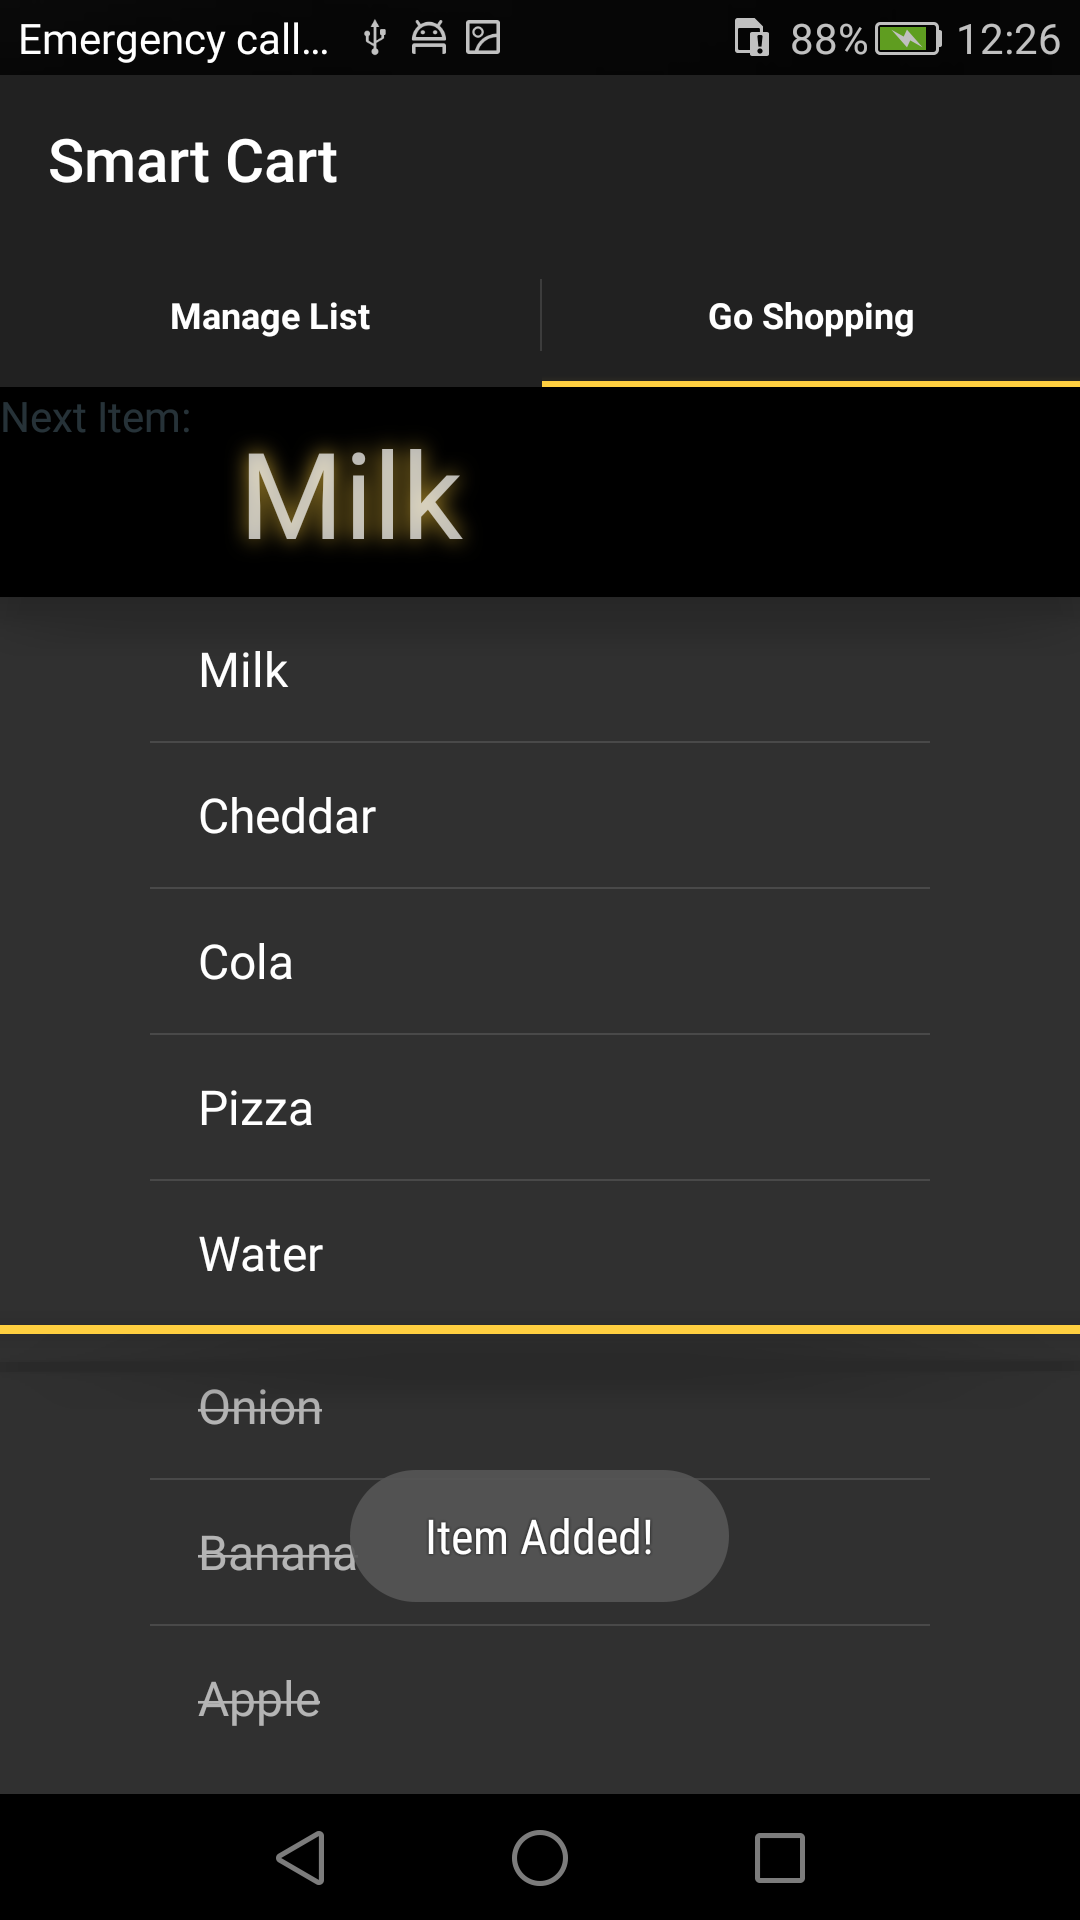
\includegraphics[width=0.8\textwidth, height=
0.35\textheight]{res/usermanual/circleRecognized.png}
\caption{Feedback Circle Recognized}
\label{fig:initial}
\end{subfigure}
\caption{Check Off Items}
\label{fig:checkItems}
\end{figure}


\begin{figure}[h]
\captionsetup{justification=centering}
\begin{subfigure}{0.475\textwidth} 
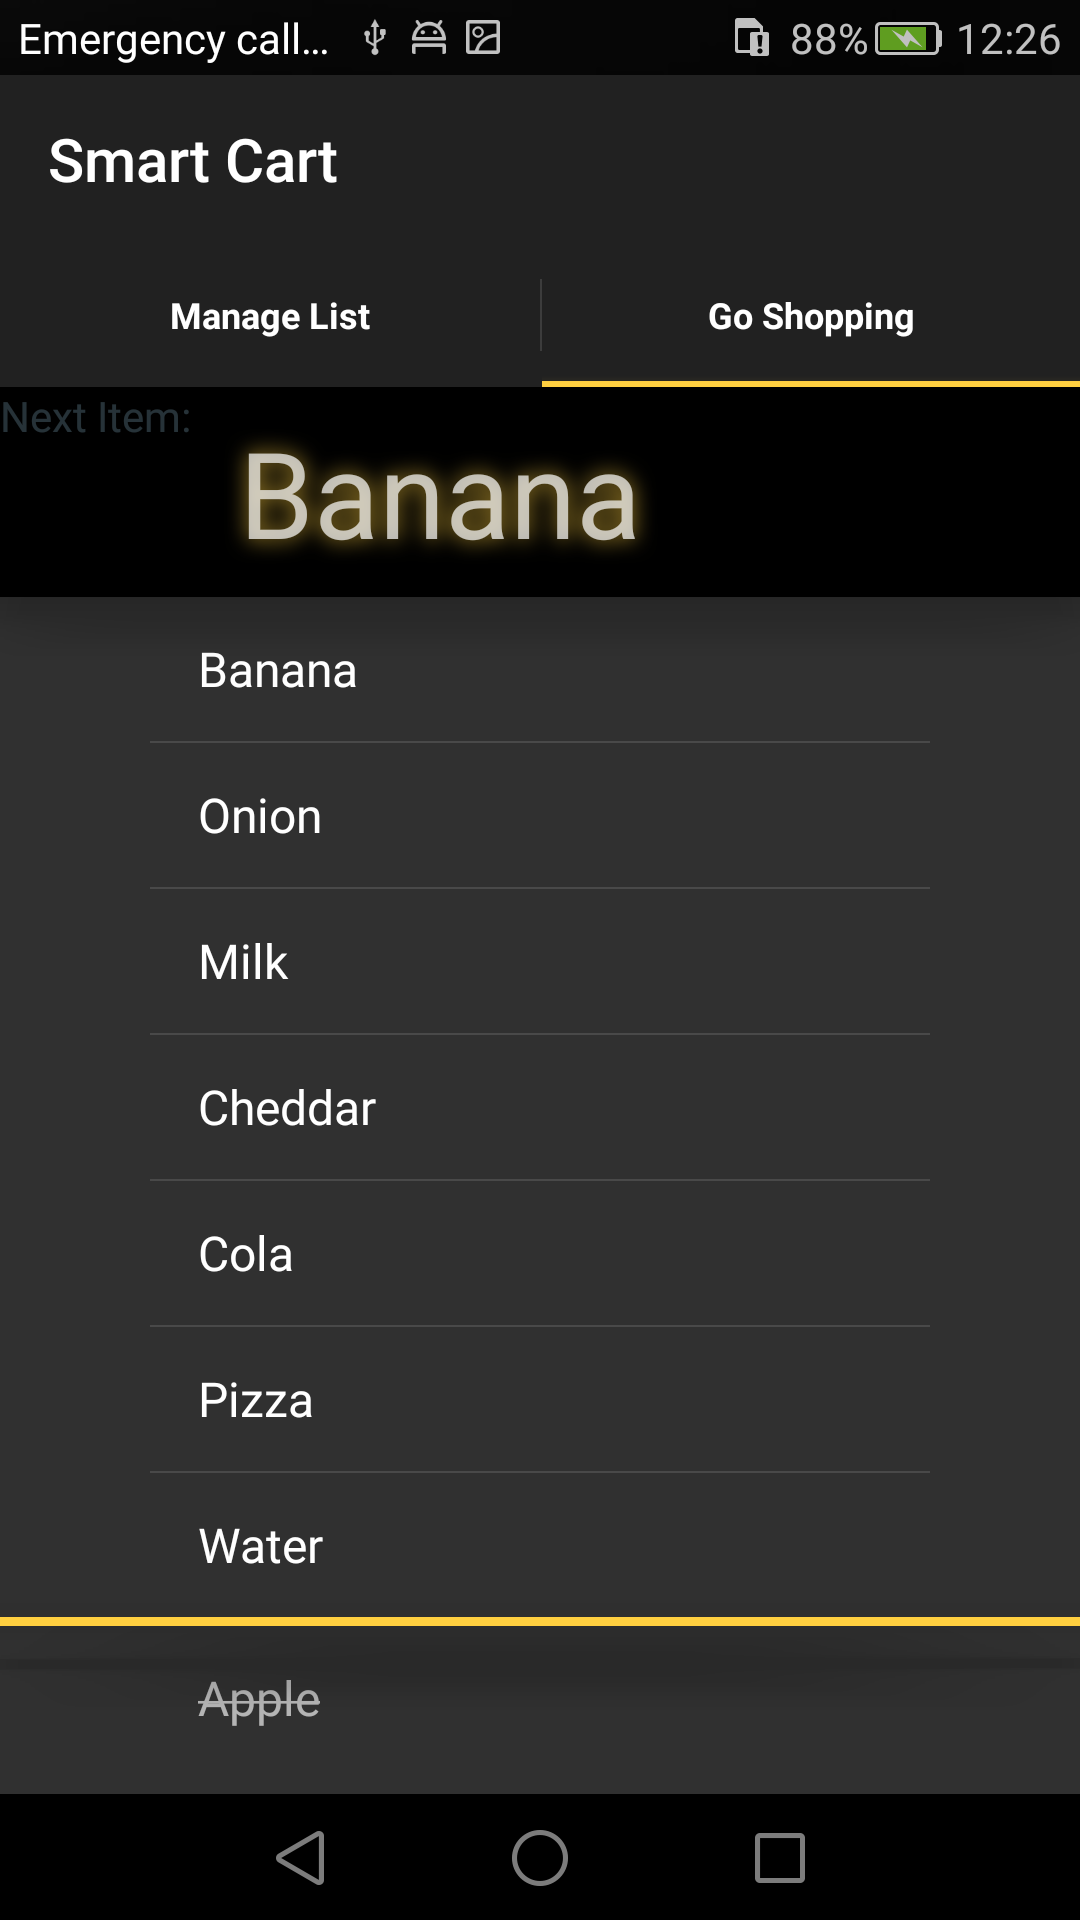
\includegraphics[width=0.8\textwidth, height=
0.35\textheight]{res/usermanual/firstItemChecked.png}
\caption{Shoppinglist before Switching}
\label{fig:beforeSwitching}
\end{subfigure} \hspace{0.2\textwidth}
\begin{subfigure}{0.475\textwidth}
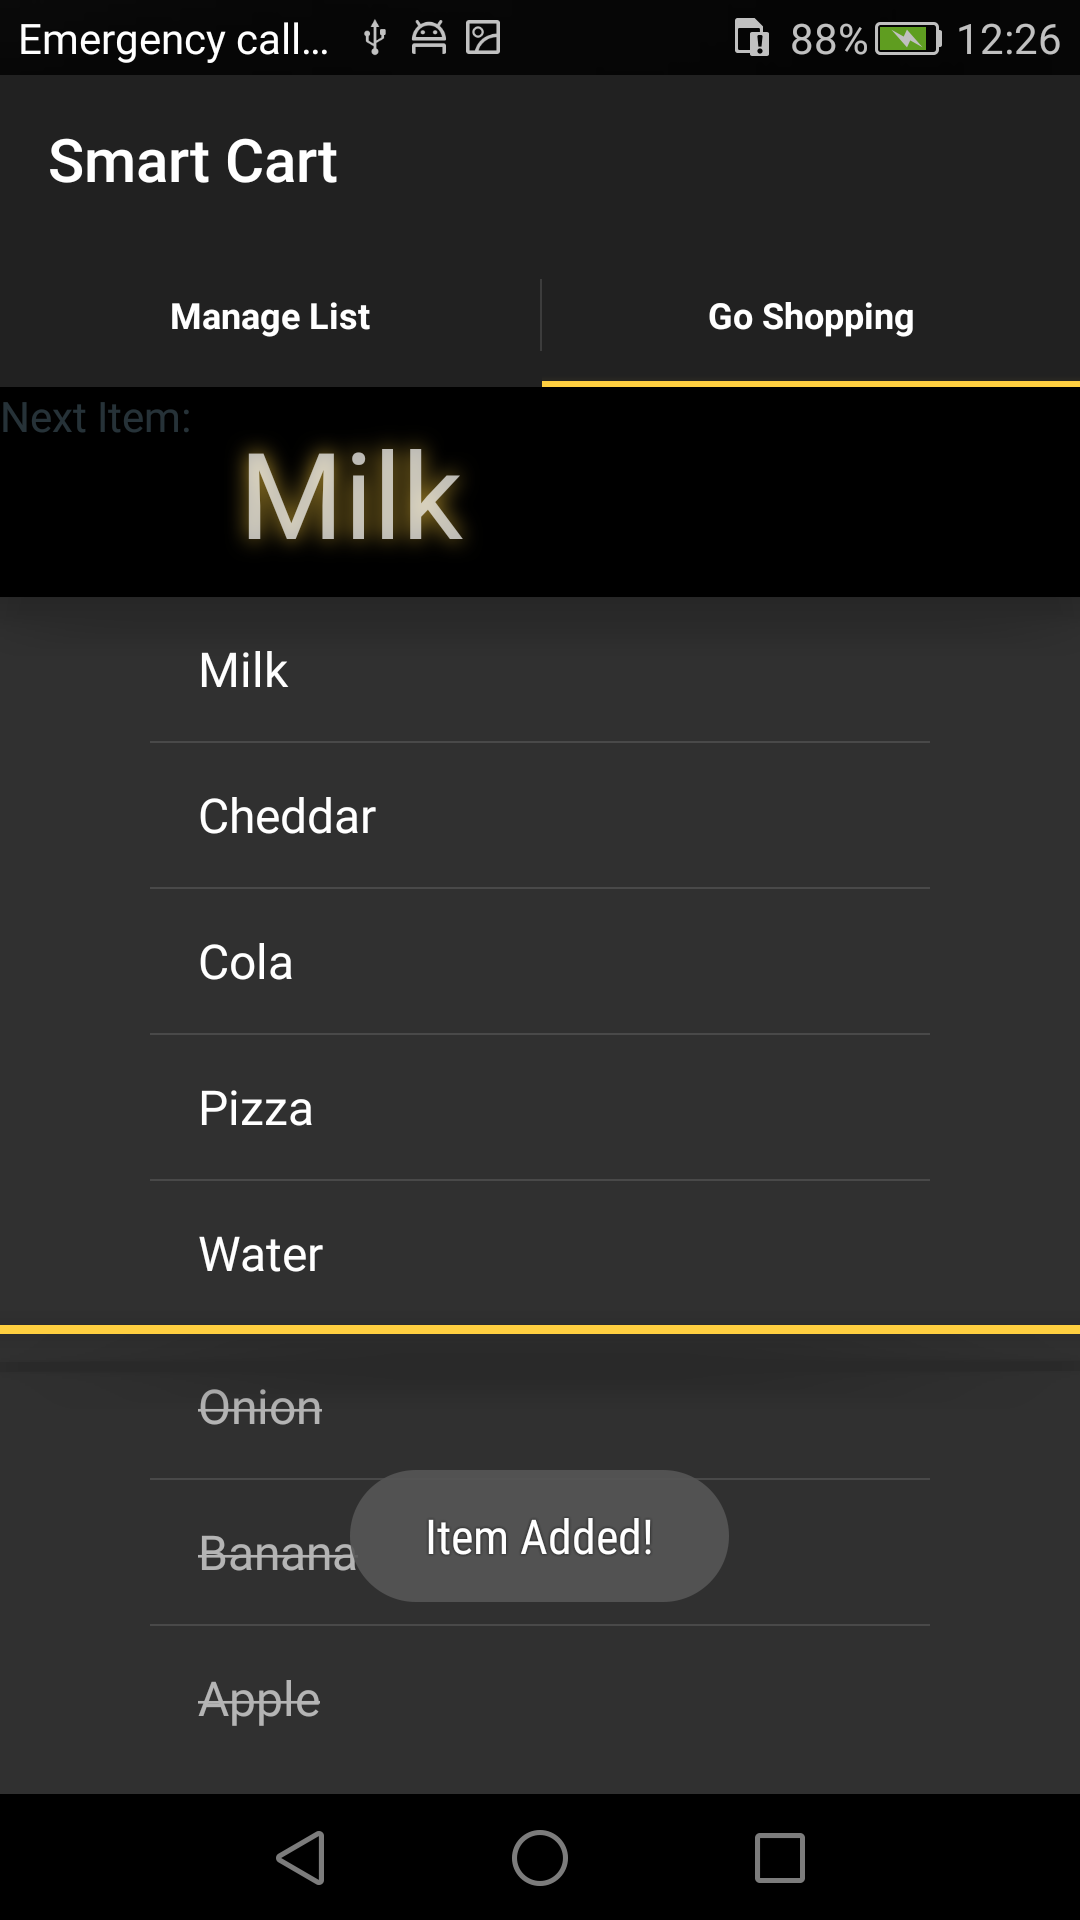
\includegraphics[width=0.8\textwidth, height=
0.35\textheight]{res/usermanual/circleRecognized.png}
\caption{Shoppinglist after Switching}
\label{fig:afterSwitching}
\end{subfigure}
\caption{Switch Items}
\label{fig:checkItems}
\end{figure}

\FloatBarrier

\subsection{Conclusion}

